% Enable warnings about problematic code
\RequirePackage[l2tabu, orthodox]{nag}
\documentclass{WeSTassignment}

\usepackage{listings}
\usepackage{color}

\definecolor{dkgreen}{rgb}{0,0.6,0}
\definecolor{gray}{rgb}{0.5,0.5,0.5}
\definecolor{mauve}{rgb}{0.58,0,0.82}

\lstset{frame=tb,
  language=python,
  aboveskip=3mm,
  belowskip=3mm,
  showstringspaces=false,
  columns=flexible,
  basicstyle={\small\ttfamily},
  numbers=none,
  numberstyle=\tiny\color{gray},
  keywordstyle=\color{blue},
  commentstyle=\color{dkgreen},
  stringstyle=\color{mauve},
  breaklines=true,
  breakatwhitespace=true,
  tabsize=2
}


% The lecture title, e.g. "Web Information Retrieval".
\lecture{Introduction to Web Science}
% The names of the lecturer and the instructor(s)
\author{%
  Prof. Dr.~Steffen~Staab\\{\normalsize\mailto{staab@uni-koblenz.de}} \and
  Ren{\'e}~Pickhardt\\{\normalsize\mailto{rpickhardt@uni-koblenz.de}} \and
   Korok~Sengupta\\{\normalsize\mailto{koroksengupta@uni-koblenz.de}} \and 
   Olga~Zagovora\\{\normalsize\mailto{zagovora@uni-koblenz.de}}
}
% Assignment number.
\assignmentnumber{7}
% Institute of lecture.
\institute{%
  Institute of Web Science and Technologies\\%
  Department of Computer Science\\%
  University of Koblenz-Landau%
}
% Date until students should submit their solutions.
\datesubmission{December 14, 2016, 10:00 a.m.}
% Date on which the assignments will be discussed in the tutorial.
\datetutorial{December 16, 2016, 12:00 p.m.}

% Set langauge of text.
\setdefaultlanguage[
  variant = american, % Use American instead of Britsh English.
]{english}

% Specify bib file location.
\addbibresource{bibliography.bib}

% For left aligned centerd boxes
% see http://tex.stackexchange.com/a/25591/75225
\usepackage{varwidth}

% ==============================================================================
% Document

\begin{document}

\maketitle
Please look at the lessons 1) \textbf{Similarity of Text} \& 2) \textbf{Generative Models}

For all the assignment questions that require you to write code, make sure to include the code in the answer sheet, along with a separate python file. Where screen shots are required, please add them in the answers directly and not as separate files.\\ \\ 

%Please mention your team Names here: 
Team Name: papa
\\Members: 
\\Brigitte Aznar
\\Bonasmitha Behura
\\Ilia Tugushi


\section{Modelling Text in a Vector Space and calculate similarity (10 points)}

Given the following three documents:

$D_1$ = this is a text about web science 

$D_2$ = web science is covering the analysis of text corpora 

$D_3$ = scientific methods are used to analyze webpages 

\subsection{Get a feeling for similarity as a human}
Without applying any modeling methods just focus on the semantics of each document and decide which two Documents should be most similar. Explain why you have this opinion in a short text using less than 500 characters. 
\\\\ \textbf{Answer:}
\\For the given documents we conclude that $D_1$ and $D_2$ are the most similar texts because it has 4 words in common (is, text, web, science). Contrary to $D_3$ which has 0 words in common with the other two documents.

\subsection{Model the documents as vectors and use the cosine similarity}
Now recall that we used vector spaces in the lecture in order to model the documents. 

\begin{enumerate}
\item How many base vectors would be needed to model the documents of this corpus?
\begin{enumerate}
\item 19 , because there are 19 unique words in all 3 documents
\end{enumerate}
\item What does each dimension of the vector space stand for?
\begin{enumerate}
\item Every dimension is a word (unique) in the document
\end{enumerate}
\item How many dimensions does the vector space have? 
\begin{enumerate}
\item There are 19 unique words in all 3 documents, so this is the number of dimensions of the vector space.
\end{enumerate}
\item Create a table to map words of the documents to the base vectors.\\
\begin{tabular}{ | l | r | }
\hline
  this & $(1,0,0,0,0,0,0,0,0,0,0,0,0,0,0,0,0,0,0)^{T}$ \\ \hline
  is & $(0,1,0,0,0,0,0,0,0,0,0,0,0,0,0,0,0,0,0)^{T}$ \\ \hline
  a & $(0,0,1,0,0,0,0,0,0,0,0,0,0,0,0,0,0,0,0)^{T}$\\ \hline
  text & $(0,0,0,1,0,0,0,0,0,0,0,0,0,0,0,0,0,0,0)^{T}$\\ \hline
  about & $(0,0,0,0,1,0,0,0,0,0,0,0,0,0,0,0,0,0,0)^{T}$\\ \hline
  web & $(0,0,0,0,0,1,0,0,0,0,0,0,0,0,0,0,0,0,0)^{T}$\\ \hline
  science & $(0,0,0,0,0,0,1,0,0,0,0,0,0,0,0,0,0,0,0)^{T}$\\ \hline
  covering & $(0,0,0,0,0,0,0,1,0,0,0,0,0,0,0,0,0,0,0)^{T}$ \\ \hline
  the & $(0,0,0,0,0,0,0,0,1,0,0,0,0,0,0,0,0,0,0)^{T}$\\ \hline
  analysis & $(0,0,0,0,0,0,0,0,0,1,0,0,0,0,0,0,0,0,0)^{T}$ \\ \hline
  of & $(0,0,0,0,0,0,0,0,0,0,1,0,0,0,0,0,0,0,0)^{T}$\\ \hline
  corpora & $(0,0,0,0,0,0,0,0,0,0,0,1,0,0,0,0,0,0,0)^{T}$\\ \hline
  scientific & $(0,0,0,0,0,0,0,0,0,0,0,0,1,0,0,0,0,0,0)^{T}$\\ \hline
  methods & $(0,0,0,0,0,0,0,0,0,0,0,0,0,1,0,0,0,0,0)^{T}$\\ \hline
  are & $(0,0,0,0,0,0,0,0,0,0,0,0,0,0,1,0,0,0,0)^{T}$\\ \hline
  used & $(0,0,0,0,0,0,0,0,0,0,0,0,0,0,0,1,0,0,0)^{T}$ \\ \hline
  to & $(0,0,0,0,0,0,0,0,0,0,0,0,0,0,0,0,1,0,0)^{T}$\\ \hline
  analyze & $(0,0,0,0,0,0,0,0,0,0,0,0,0,0,0,0,0,1,0)^{T}$ \\ \hline
  webpages & $(0,0,0,0,0,0,0,0,0,0,0,0,0,0,0,0,0,0,1)^{T}$\\
  \hline
\end{tabular}
\item Use the notation and formulas from the lecture to represent the documents as document vectors in the word vector space. You can use the term frequency of the words as coefficients. You can / should omit the inverse document frequency.
\begin{enumerate}
\item  $D_1$ = this is a text about web science 
\\ $\vec{d_1}$ = 1 x $(1,0,0,0,0,0,0,0,0,0,0,0,0,0,0,0,0,0,0)^{T}$ + 1 x $(0,1,0,0,0,0,0,0,0,0,0,0,0,0,0,0,0,0,0)^{T}$ + 1 x $(0,0,1,0,0,0,0,0,0,0,0,0,0,0,0,0,0,0,0)^{T}$ + 1 x$(0,0,0,1,0,0,0,0,0,0,0,0,0,0,0,0,0,0,0)^{T}$ + 1 x $(0,0,0,0,1,0,0,0,0,0,0,0,0,0,0,0,0,0,0)^{T}$ + 1 x
$(0,0,0,0,0,1,0,0,0,0,0,0,0,0,0,0,0,0,0)^{T}$ + 1 x 
$(0,0,0,0,0,0,1,0,0,0,0,0,0,0,0,0,0,0,0)^{T}$ =
\\$(1,1,1,1,1,1,1,0,0,0,0,0,0,0,0,0,0,0,0)^{T}$
\\\\  $\vec{d_2}$ = 1 x $(0,0,0,0,0,1,0,0,0,0,0,0,0,0,0,0,0,0,0)^{T}$ + 1 x 
$(0,0,0,0,0,0,1,0,0,0,0,0,0,0,0,0,0,0,0)^{T}$ + 1 x $(0,1,0,0,0,0,0,0,0,0,0,0,0,0,0,0,0,0,0)^{T}$ + 1 x$(0,0,0,0,0,0,0,1,0,0,0,0,0,0,0,0,0,0,0)^{T}$ + 1 x  $(0,0,0,0,0,0,0,0,1,0,0,0,0,0,0,0,0,0,0)^{T}$ + 1 x $(0,0,0,0,0,0,0,0,0,1,0,0,0,0,0,0,0,0,0)^{T}$ + 1 x
$(0,0,0,0,0,0,0,0,0,0,1,0,0,0,0,0,0,0,0)^{T}$ + 1 x
$(0,0,0,1,0,0,0,0,0,0,0,0,0,0,0,0,0,0,0)^{T}$ + 1 x $(0,0,0,0,0,0,0,0,0,0,0,1,0,0,0,0,0,0,0)^{T}$ = 
\\$(0,1,0,1,0,1,1,1,1,1,1,1,0,0,0,0,0,0,0)^{T}$
\\\\  $\vec{d_3}$ = 1 x $(0,0,0,0,0,0,0,0,0,0,0,0,1,0,0,0,0,0,0)^{T}$ + 1 x $(0,0,0,0,0,0,0,0,0,0,0,0,0,1,0,0,0,0,0)^{T}$ + 1 x $(0,0,0,0,0,0,0,0,0,0,0,0,0,0,1,0,0,0,0)^{T}$ + 1 x $(0,0,0,0,0,0,0,0,0,0,0,0,0,0,0,1,0,0,0)^{T}$ + 1 x  $(0,0,0,0,0,0,0,0,0,0,0,0,0,0,0,0,1,0,0)^{T}$ + 1 x $(0,0,0,0,0,0,0,0,0,0,0,0,0,0,0,0,0,1,0)^{T}$ + 1 x $(0,0,0,0,0,0,0,0,0,0,0,0,0,0,0,0,0,0,1)^{T}$ = 
\\$(0,0,0,0,0,0,0,0,0,0,0,0,1,1,1,1,1,1,1)^{T}$
\end{enumerate}
\item Calculate the cosine similarity between all three pairs of vectors.
\begin{figure}[h]
  \centering
  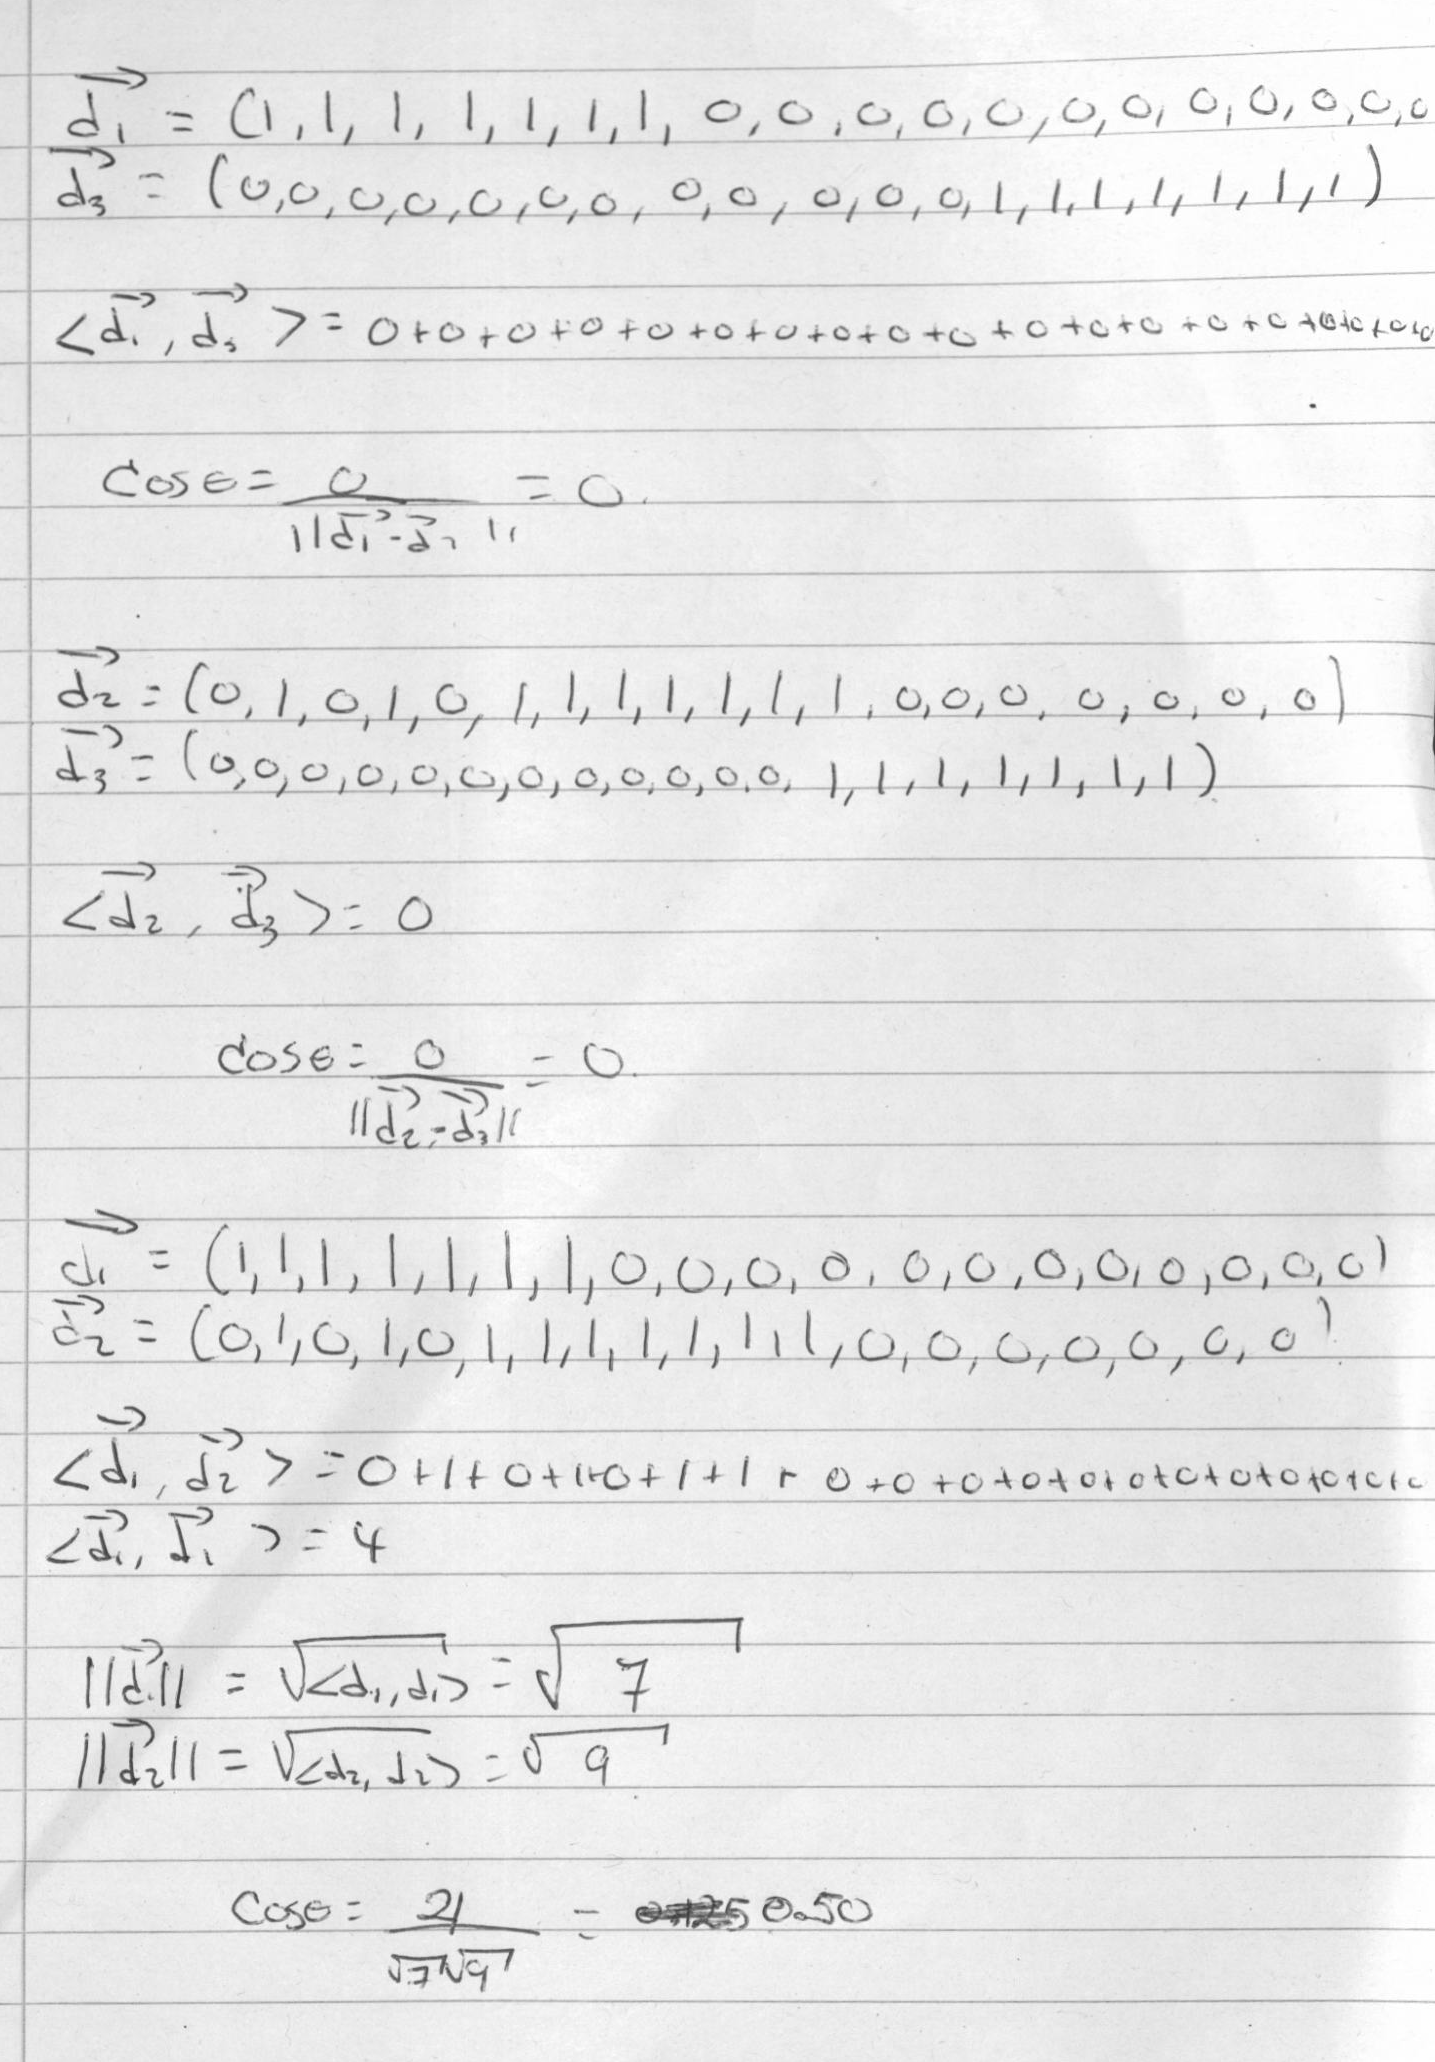
\includegraphics[scale=0.5]{exercise1.png}
   \caption{Calculations for the cosine similarity}
     \label{fig:dig} 
\end{figure}
\item According to the cosine similarity which 2 documents are most similar according to the constructed model. 
\begin{enumerate}
\item $D_1$ and $D_2$ are the more similar documents with a similarity of \textbf{.50} according to the cosine similarity
\end{enumerate}
\end{enumerate}

\subsection{Discussion}
Do the results of the model match your expectations from the first subtask? If yes explain why the vector space matches the similarity given from the semantics of the documents. If no explain what the model lacks to take into consideration. Again 500 Words should be enough. 
\\ The space vector does match our expectations, this is because in documents 1 and 2 there are some words in common which gives some sense of similarity to the documents, unlike document 3 which has no word in common, which nullifies the denominator in the division and makes the similarity equals to 0.


%-------------------------------------------------------------------------------

\section{Building generative models and compare them to the observed data (10 points)}
This week we provide you with two probability distributions for characters and spaces which can be found next to the exercise sheet on the WeST website. Also last week we provided you with a dump of Simple English Wikipedia which should be reused this week.

\subsection{build a generator}
Count the characters and spaces in the Simple English Wikipedia dump. Let the combined number be $n$. 
Use the sampling method from the lecture to sample $n$ characters (which could be letters or a space) from each distribution.
Store the result for the generated text for each distribution in a file.

\subsection{Plot the word rank frequency diagram and CDF}
Count the resulting words from the provided data set and from the generated text for each of the probability distributions. 
Create a word rank frequency diagram which contains all 3 data sets. 
Also create a CDF plot that contains all three data sets. 

\subsection{Which generator is closer to the original data?}
Let us assume you would want to creat a test corpus for some experiments. That test corpus has to have a similar word rank frequency diagram as the original data set. Which of the two generators would you use? You should perform the Kolmogorov Smirnov test as discussed in the lecture by calculating the maximum pointwise distance of the CDFs. \\

\textbf{Answer:}
\\ We would use the Zipf generator, because the distribution of characters is not uniform (which is the case with real texts) and also becasue it includes alphanumeric values which our base text also contains.
\\ The result of substracting the max two data points for the zipf distribution is smaller than the uniform distribution, which means it is a little closer to the base text.


\textbf{How do your results change when you generate the two text corpora for a second or third time? What will be the values of the Kolmogorov Smirnov test in these cases?}\\

\textbf{Answers:}
\\The Kolmogorov Smirnov test is the same for the 3 times we ran the code, The graphics didn't change either, this is because the same pattern is repeated and therfore gives very similar results. In the pictures below are the resulting graphics

\subsection{Hints:}
\begin{enumerate}
\item Build the cummulative distribution function for the text corpus and the two generated corpora
\item Calculate the maximum pointwise distance on the resulting CDFs
\item You can use \texttt{Collections.Counter}, \texttt{matplotlib} and \texttt{numpy}. You shouldn't need other libs. \\
\end{enumerate}
\textbf{Answers: }
\begin{lstlisting}
import os
import re
import random
import numpy as np
import matplotlib.pyplot as plt
import matplotlib.patches as mpatches
from collections import Counter

def ReadWiki():
    path_to_file = os.path.realpath('.')
    n = 0
    with open(os.path.join(path_to_file, 'simple_english_wikipedia.txt'), encoding="utf8") as file:
        for line in file:
            for char in line:
                if re.findall('([A-Z a-z ])', char):#any latin letter(cap or lower case) and spaces
                    n += 1
    return n

def CalculateZipf():
    zipf = {}
    probs_new = 0
    zipf_probabilities = {' ': 0.17840450037213465, '1': 0.004478392057619917,
                          '0': 0.003671824660673643, '3': 0.0011831834225755678,
                          '2': 0.0026051307175779174, '5': 0.0011916662329062454,
                          '4': 0.0011108979455528355, '7': 0.001079651630435706,
                          '6': 0.0010859164582487295, '9': 0.0026071152282516083,
                          '8': 0.0012921888323905763, '_': 2.3580656240324293e-05,
                          'a': 0.07264712490903191, 'c': 0.02563767289222365,
                          'b': 0.013368688579962115, 'e': 0.09688273452496411,
                          'd': 0.029857183586861923, 'g': 0.015076820473031856,
                          'f': 0.017232219565845877, 'i': 0.06007894642873102,
                          'h': 0.03934894249122837, 'k': 0.006067466280926215,
                          'j': 0.0018537015877810488, 'm': 0.022165129421030945,
                          'l': 0.03389465109649857, 'o': 0.05792847618595622,
                          'n': 0.058519445305660105, 'q': 0.0006185966212395744,
                          'p': 0.016245321110753712, 's': 0.055506530071283755,
                          'r': 0.05221605572640867, 'u': 0.020582942617121572,
                          't': 0.06805204881206219, 'w': 0.013964469813783246,
                          'v': 0.007927199224676324, 'y': 0.013084644140464391,
                          'x': 0.0014600810295164054, 'z': 0.001048859288348506}
    for char, prob in zipf_probabilities.items():
        probs_new += prob
        zipf[char] = probs_new
    return zipf

def CalculateUniform():
    uniform = {}
    probs_new = 0
    uniform_probabilities = {' ': 0.1875, 'a': 0.03125, 'c': 0.03125, 'b': 0.03125, 'e': 0.03125, 'd': 0.03125,
                             'g': 0.03125, 'f': 0.03125, 'i': 0.03125, 'h': 0.03125, 'k': 0.03125, 'j': 0.03125,
                             'm': 0.03125, 'l': 0.03125, 'o': 0.03125, 'n': 0.03125, 'q': 0.03125, 'p': 0.03125,
                             's': 0.03125, 'r': 0.03125, 'u': 0.03125, 't': 0.03125, 'w': 0.03125, 'v': 0.03125,
                             'y': 0.03125, 'x': 0.03125, 'z': 0.03125}

    for char, prob in uniform_probabilities.items():
          probs_new += prob
          uniform[char] = probs_new
    return uniform

def makeGibberish(prob, n, prob_name):
    i = 0
    words = ''
    find_char = []
    while i <= n:
        i += 1
        rand = random.random()
        for key, val in prob.items():
            if val >= rand:
                find_char.append(val)
        try:
            next_char_val = min(find_char) #finds the closest (smaller) value of the probability model to rand
        except(Exception):
            print('somethin went worng')
            pass

        for char, val in prob.items():
            if next_char_val == val:
                next_char = char

        find_char = [] #reinitializes the array
        words += next_char
    saveFile(words, prob_name)

def saveFile(words, file_name):
    path_to_file = os.path.realpath('.')
    with open(os.path.join(path_to_file, file_name+'.txt'), 'w') as file_to_write:
        file_to_write.write(words)
        file_to_write.close()

def countWords(file):
    path_to_file = os.path.realpath('.')
    total_words = 0
    words = []
    with open(os.path.join(path_to_file, file), encoding="utf8") as file:
        for line in file:
            total_words += len(re.findall(r'\w+', line))
            words += re.findall(r'\w+', line)

    return words, total_words

def rank(words, do_join):
    if do_join:
        words = ' '.join(words)
    counter = Counter(words)
    words, frq = zip(*counter.most_common())

    return frq

def rankPlot(x_zipf, x_uniform, x_sew, zipf_freq, uniform_freq, sew_freq):

    plt.loglog(x_zipf, zipf_freq, 'r-')
    plt.loglog(x_uniform, uniform_freq, 'b-')
    plt.loglog(x_sew, sew_freq, 'g-')

    # adds labels to the axis
    plt.ylabel('Frequency')
    plt.xlabel('Word Rank')
    # generates legend
    zipf_legend = mpatches.Patch(color='red', label='generated zipf')
    unifrom_legend = mpatches.Patch(color='blue', label='generated uniform')
    sew_legend = mpatches.Patch(color='green', label='original text')
    plt.legend(handles=[zipf_legend, unifrom_legend,sew_legend ], loc=5)
    plt.show()

def getCDF(freq):
    cumsum = np.cumsum(freq)
    normedcumsum = [x/float(cumsum[-1]) for x in cumsum]
    return normedcumsum

def plotCDF(x_zipf, x_uniform, x_sew, zipf_cumsum, uniform_cumsum, sew_cumsum):
    plt.semilogx(x_zipf, zipf_cumsum, 'r-')
    plt.semilogx(x_uniform, uniform_cumsum, 'b-')
    plt.semilogx(x_sew, sew_cumsum, 'g-')

    # adds labels to the axis
    plt.ylabel('CDF')
    plt.xlabel('Word Rank')
    # generates legend
    zipf_legend = mpatches.Patch(color='red', label='generated zipf')
    unifrom_legend = mpatches.Patch(color='blue', label='generated uniform')
    sew_legend = mpatches.Patch(color='green', label='original text')
    plt.legend(handles=[zipf_legend, unifrom_legend, sew_legend], loc=5)
    plt.show()

def task(zip_file, uniform_file):
    path_to_file = os.path.realpath('.')
    print('Counting chars in SEW please wait')
    #n = read_wiki() #89860319 number of letters and spaces
    n = 89860319
    zipf = CalculateZipf()
    uniform = CalculateUniform()

    if not os.path.isfile(os.path.join(path_to_file,zip_file + '.txt')):
        print('Starting gibberish creation from zipf')
        makeGibberish(zipf, n, zip_file)
        print(zip_file + '.txt Created')

    if not os.path.isfile(uniform_file + '.txt'):
        print('Starting gibberish creation from uniform probabilities')
        makeGibberish(uniform, n, uniform_file)
        print(uniform_file + '.txt Created')

    print('Starting Word count for zipf distribution')
    zipf_words, zipf_count = countWords(zip_file + '.txt')
    print(zipf_count)

    print('Starting Word count for uniform distribution')
    uniform_words, uniform_count = countWords(uniform_file + '.txt')
    print(uniform_count)

    print('Starting Word count for SEW')
    sew_words, sew_count = countWords('simple_english_wikipedia.txt')
    print(sew_count)
    
    print('Calculating rank of zip')
    zipf_frq = rank(zipf_words, False)

    print('Calculating rank of uniform')
    uniform_frq = rank(uniform_words, False)

    print('Calculating rank of sew')
    sew_frq = rank(sew_words, True)
    x_zipf = [i for i in range(0, len(zipf_frq))]
    x_uniform = [i for i in range(0, len(uniform_frq))]
    x_sew = [i for i in range(0, len(sew_frq))]

    print('Generating plot')
    rankPlot(x_zipf, x_uniform, x_sew, zipf_frq, uniform_frq, sew_frq)
    print('Calculating CDF for Zipf')
    zipf_cdf_cumsum = getCDF(zipf_frq)

    print('Calculating CDF for uniform')
    uniform_cdf_cumsum = getCDF(uniform_frq)

    print('Calculating CDF for SEW')
    sew_cdf_cumsum = getCDF(sew_frq)

    x_zipf = [i for i in range(0, len(zipf_cdf_cumsum))]
    x_uniform = [i for i in range(0, len(uniform_cdf_cumsum))]
    x_sew = [i for i in range(0, len(sew_cdf_cumsum))]
    
    print('Generating CDF plot')
    plotCDF(x_zipf, x_uniform, x_sew, zipf_cdf_cumsum, uniform_cdf_cumsum, sew_cdf_cumsum)
    
    #Kolmogorv Smirnov test 
    smirnov_zipf_max=[]
    zipf_cdf_cumsum = zipf_cdf_cumsum [0:len(sew_cdf_cumsum)]
    smirnov_zipf = [sew_cdf_cumsum_i - zipf_cdf_cumsum_i for sew_cdf_cumsum_i, zipf_cdf_cumsum_i in zip(sew_cdf_cumsum, zipf_cdf_cumsum)]
    smirnov_zipf_max.append(max(smirnov_zipf))
    print(smirnov_zipf_max)

    #Kolmogorv Smirnov test 
    smirnov_uniform_max= []
    uniform_cdf_cumsum = uniform_cdf_cumsum [0:len(sew_cdf_cumsum)]
    uniform_zipf = [sew_cdf_cumsum_i - uniform_cdf_cumsum_i for sew_cdf_cumsum_i, uniform_cdf_cumsum_i in zip(sew_cdf_cumsum, uniform_cdf_cumsum)]
    smirnov_uniform_max.append(max(uniform_zipf))
    print(smirnov_uniform_max)
    

def main():
   task("zipf", 'uniform',)
   task('zipf_2', 'uniform_2')
   task('zipf_3', 'uniform_3')

if __name__ == "__main__":
    main()

\end{lstlisting}

\begin{figure}[h!]
  \centering
  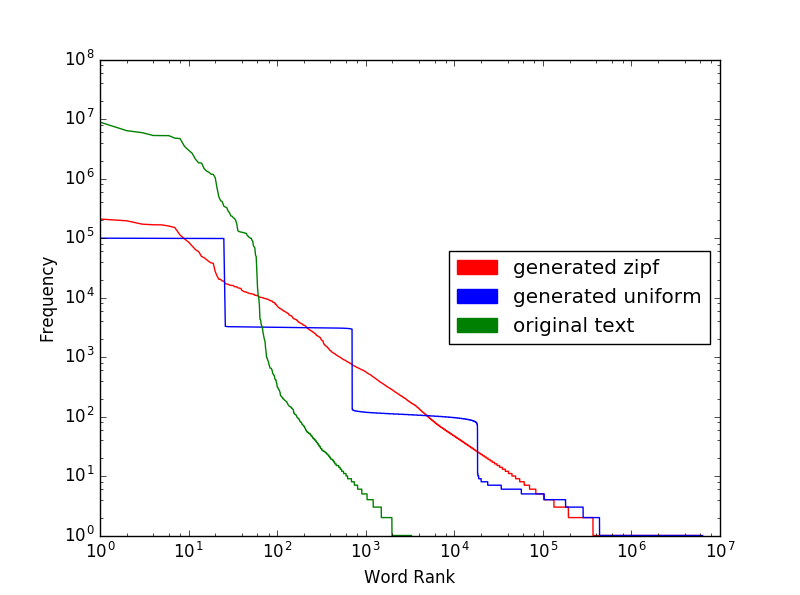
\includegraphics[scale=0.5]{word_rank_freq_1.png}
   \caption{Word rank frecuency for the first time}
     \label{fig:dig} 
\end{figure}

\begin{figure}[h!]
  \centering
  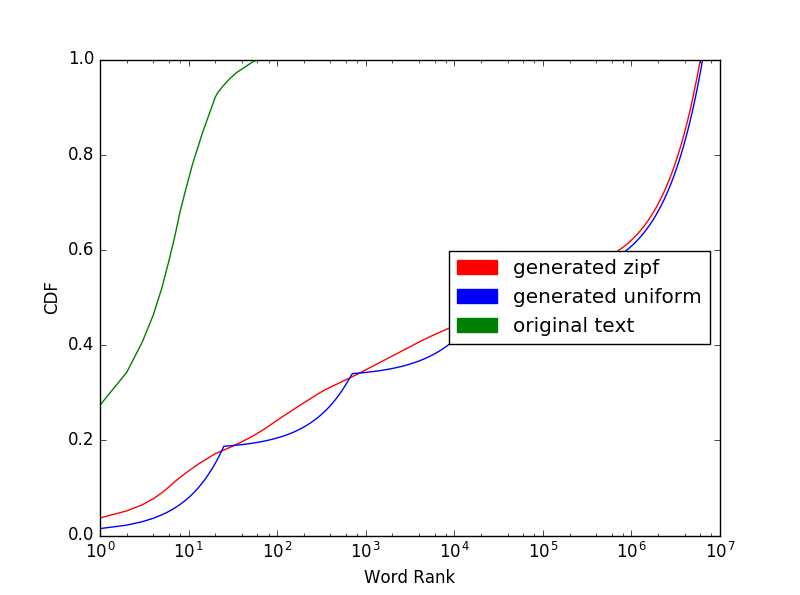
\includegraphics[scale=0.5]{cdf_1.png}
   \caption{Word rank frecuency for the first time}
     \label{fig:dig} 
\end{figure}


\begin{figure}[h!]
  \centering
  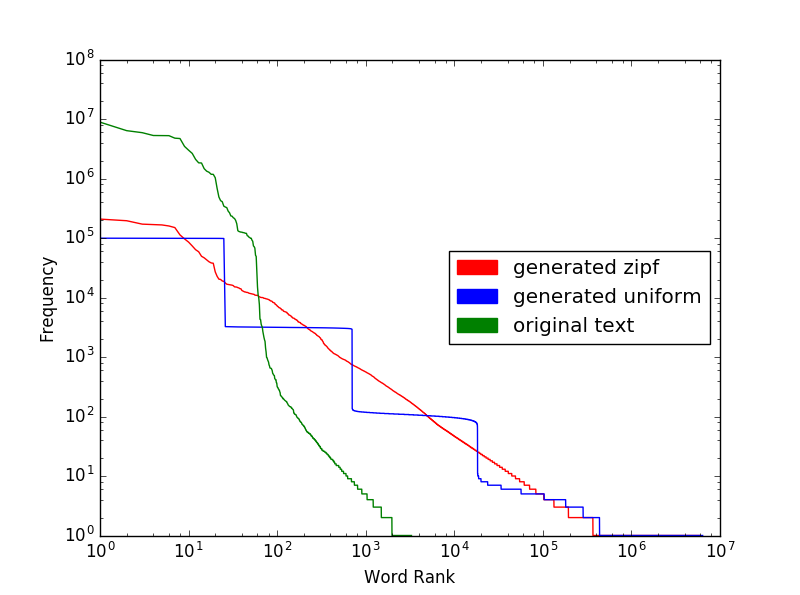
\includegraphics[scale=0.5]{word_rank_freq_2.png}
   \caption{Word rank frecuency for the second time}
     \label{fig:dig} 
\end{figure}

\begin{figure}[h!]
  \centering
  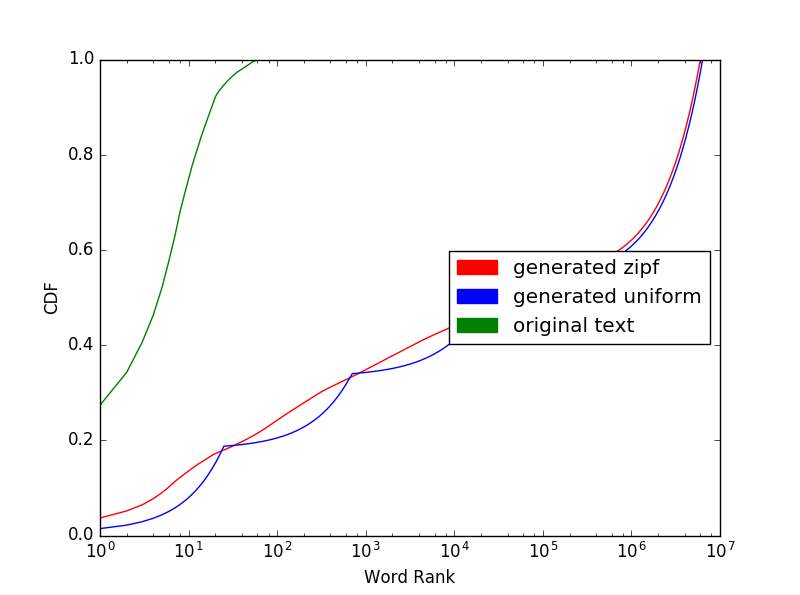
\includegraphics[scale=0.5]{cdf_2.png}
   \caption{Word rank frecuency for the second time}
     \label{fig:dig} 
\end{figure}


\begin{figure}[h!]
  \centering
  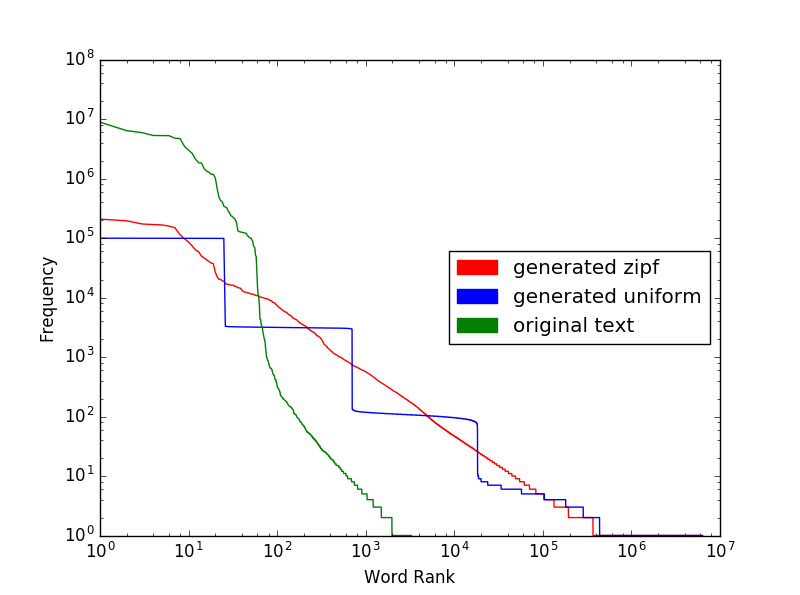
\includegraphics[scale=0.5]{word_rank_freq_3.png}
   \caption{Word rank frecuency for the third time}
     \label{fig:dig} 
\end{figure}

\begin{figure}[h!]
  \centering
  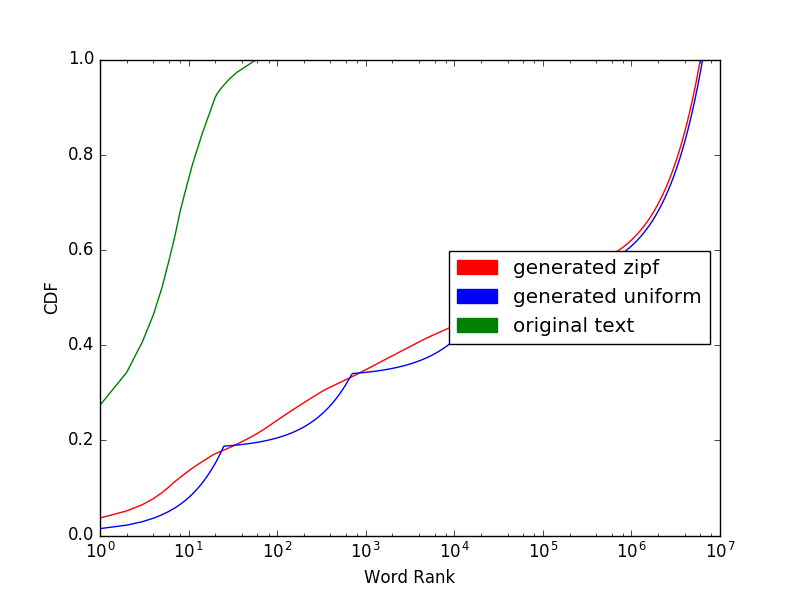
\includegraphics[scale=0.5]{cdf_3.png}
   \caption{Word rank frecuency for the third time}
     \label{fig:dig} 
\end{figure}



%-------------------------------------------------------------------------------

%-------------------------------------------------------------------------------

\section{Understanding of the cumulative distribution function (10 points)}

Write a fair 6-side die rolling simulator. A fair die is one for which each face appears with equal likelihood. Roll two dice simultaneously n (=100) times and record the sum of both dice each time. 

\begin{enumerate}
\item Plot a readable histogram with frequencies of dice sum outcomes from the simulation. 
\item Calculate and plot cumulative distribution function.
\item Answer the following questions using CDF plot:

What is the median sum of two dice sides?  Mark the point on the plot.

What is the probability of dice sum to be equal or less than 9? Mark the point on the plot.

%What are the values 
\item Repeat the simulation a second time and compute the maximum point-wise distance of both CDFs.
\item Now repeat the simulation (2 times) with n=1000 and compute the maximum point-wise distance of both CDFs.
\item What conclusion can you draw from increasing the number of steps in the simulation?  
\\ \textbf{Answer:}
\\ The maximum pointwise distance decreased from 0.019 (in 100 rolls) to 0.012 (in 1000 rolls). This is because with more rolls is more likely that the throws are more similar to each other and then the distance between them reduces 
\end{enumerate}


\subsection{Hints}
\begin{enumerate}
\item You can use function from the lecture to calculate rank and normalized cumulative sum for CDF.
\item Do not forget to give proper names of CDF plot axes or maybe even change the ticks values of x-axis. \\
\end{enumerate}
\textbf{Answers: }
\begin{lstlisting}
import os
import re
import numpy as np
import random
import matplotlib.pyplot as plt
import matplotlib.patches as mpatches
from collections import Counter

def rollDice(n):
    dice = []
    i = 1
    while i <= n:
        dice.append(random.randint(1,6))
        i += 1
    return dice

def histogram(dice_freq, max_sum):
    plt.hist(dice_freq, bins = 11, range =(2, max_sum))
    plt.title("Frequency vs Dice sum")
    plt.ylabel("Frequency")
    plt.xlabel("Dice Sum")
    plt.show()

def getFreq(dice):
    counter = Counter(dice)
    nums, frq = zip(*counter.most_common())
    return frq, nums

def getCDF(freq):
    cumsum = np.cumsum(freq)
    normedcumsum = [x/float(cumsum[-1]) for x in cumsum]
    return normedcumsum

def plotCDF(x, cumsum, median, median_cdf, prob):
    plt.plot(x, cumsum, 'r-')
    plt.axvline(median, color='b', linestyle='dashed', linewidth=2)
    plt.axhline(median_cdf, color='b', linestyle='solid', linewidth=1)
    plt.axhline(prob, color='y', linestyle='solid', linewidth=1)

    # adds labels to the axis
    plt.ylabel('Probability')
    plt.xlabel('Dice roll')

    # generates legend
    cdf_legend = mpatches.Patch(color='red', label='CDF')
    median_legend = mpatches.Patch(color='blue', label='Median')
    prob_legend = mpatches.Patch(color='yellow', label='Median')

    plt.legend(handles=[cdf_legend, median_legend, prob_legend], loc=5)
    plt.show()

def diceSums(dice_1, dice_2, n):
    i = 0
    dice = []
    while i < n:
        dice.append(dice_1[i] + dice_2[i])
        i += 1
    return dice
def getProb(n,cdf):
    i = 0
    prob = 0
    while i <= 9:
        print(cdf[i])
        prob += cdf[i]
        i += 1
    print(prob)
    return prob
def task():
    #n = 1000
    n = 100
    dice_1 = rollDice(n)
    dice_2 = rollDice(n)
    dice = diceSums(dice_1, dice_2, n)

    max_sum = max(dice)
    histogram(dice, max_sum)

    freq, nums = getFreq(dice)

    cdf = getCDF(freq)
    x = [i for i in range(2, len(cdf) + 2)]

    median = np.median(dice)
    median_cdf = np.median(cdf)
    prob_9= cdf[9]

    plotCDF(x, cdf, median, median_cdf, prob_9)
    return cdf
def main():
    cdf_1 = task()
    cdf_2 = task()
    smirnov_max = []
    smirnov = [cdf_1_i - cdf_2_i for cdf_1_i, cdf_2_i in zip(cdf_1, cdf_2)]
    smirnov_max.append(max(smirnov))
    print(smirnov_max)
    #For 100 vals 0.059
    #For 1000 vals 0.012
if __name__ == "__main__":
        main()
\end{lstlisting}

\begin{figure}[h!]
  \centering
  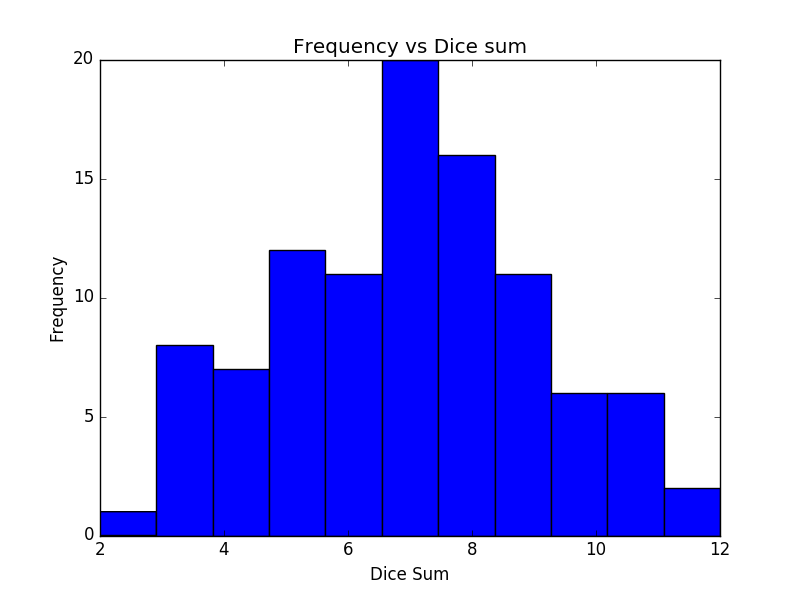
\includegraphics[scale=0.5]{histogram_100.png}
   \caption{Histogram for throwing 2 dices 100 times}
     \label{fig:dig} 
\end{figure}

\begin{figure}[h!]
  \centering
  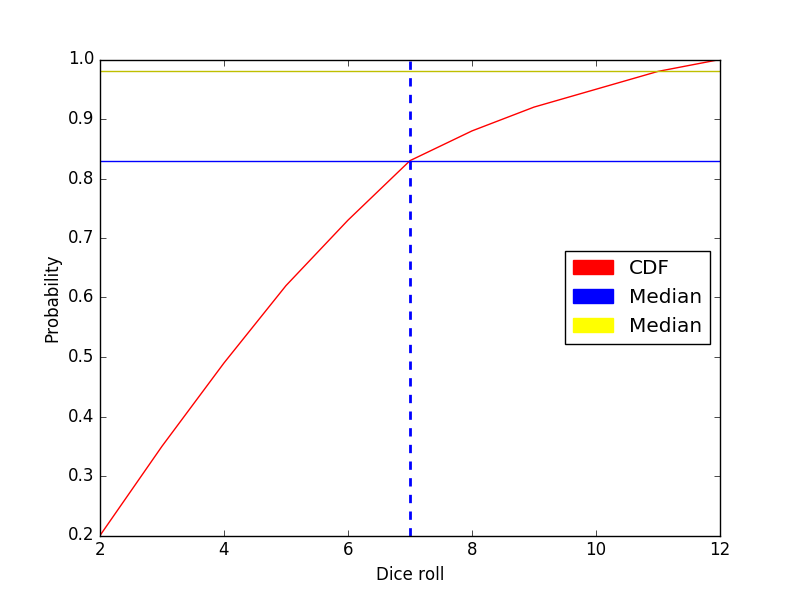
\includegraphics[scale=0.5]{dice_med_prob.png}
   \caption{Cumulative distribution function with means and prob. of 9}
     \label{fig:dig} 
\end{figure}


\subsection{Only for nerds and board students (0 Points)}
Assuming 20 groups of students. What is the likelihood that at least two groups come up with the same histograms in the case for n (=100)?





\makefooter

\end{document}
